Die erzeugten thermischen Neutronen %ref dazupacken auzs therorie
werden auf den Werkstoff gelenkt. Die anschließende auftrentende Strahlung wir von  dem Geiger-Müller-Zählrohr detektiert und mit den Zählern erfasst.
Durch die zwei Anzeigen der Zähller kann man nun die Ausgewertete Anazhl an Zerfällen ablesen, wärend der Zeitgeber automatisch nach $\Delta t$ auf die Zweite Anzeige wechselt.
Dieser Vorgamg wiederholt sich periodisch. Es lassen sich also ohne Pause genaue Messungen erzielen.

\begin{figure}
  \centering
  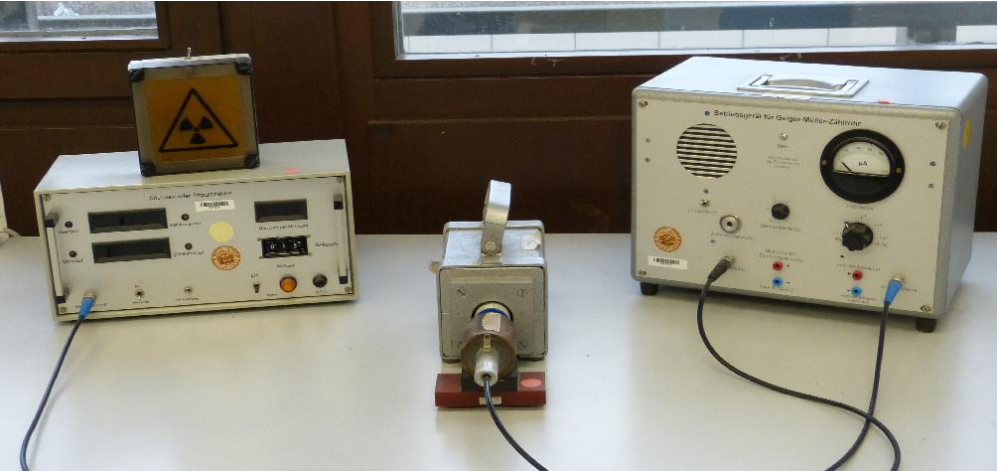
\includegraphics[width=0.8\textwidth]{bilder/Screenshot 2021-01-22 103203.png}
  \caption{Aufbau  \cite{hinweis}.}
  \label{fig:aufbau}
\end{figure}

Der Zeitgeber hat eine Genauigkeit von $\si{e-5}$ auf das Gegebene Messintervall $\Delta t$.
Zusätlich wird vor Beginn der Durchführung mit radiaktiven Substanzen der \textbf{Nulleffekt} $N_U$ %\ref zur theorie 
gemessen um ungewollte Strahlung nacher vom Ergbenis abziehen zu können.  Der Messung liegt ein statistischer Fehler bei, weswegen sich möglichst lange Messungen des Nulleffekts empfehlen.
\\
\newline
Beide Probem, Vandaium und Rhoidum, werden unmittelbar nach der Aktivierung der Neutronen dem Geiger-Müller-Zählrohr zur Messung gegeben.
Die Intervall untescheiden sich dahingehend, dass bei Vadium im INtervall von 30 Sekunden und bei Rhoidum im INtervall von 15 Sekunden gemessen wird.


